\documentclass[a4paper]{article} 
\usepackage[utf8]{inputenc}
\usepackage{parskip} 
\usepackage{graphicx}
\usepackage{amsmath}
\usepackage{biblatex}
\addbibresource{sources.bib}

\title{Techniques in Functional Programming\\
Term Project\\
Fold right and fold left}
\author{Benjamin Nørgaard \#201209884}
\date{April 2015}

\begin{document}

\maketitle
\tableofcontents
\clearpage
\section{Introduction}
This project explores the functions \texttt{fold\_right} and
\texttt{fold\_left}. In order to understand what the fold functions do and how
they work, we will define a few functions using folds. We will then see if we
can define one fold function in term of the other. We will find that there are
some cases where it does not make any difference whether we use
\texttt{fold\_right} or \texttt{fold\_left}, and we will try to formalise when
this applies. In the end we will draw parallels to primitive iteration and
primitive recursion.

\subsection{About this report}
This report was written to document a project written using Coq Proof Assistant.
The report is meant to be read alongside the actual Coq source file. There will
not be be code in the report, but I will instead refer to and talk about the
code written in the source file.

\subsection{About the source file}
The source file is long, but it is structured more or less like the sections in
this report, so it should be easy enough to follow along in the code.

We use a few conventions in the source code. Most noticeably is the meaning of
the indentation: Proofs are indented by two spaces per subgoal. This makes it
easier to for example see the cases of an induction proof visually in the
indentation.

The code has quite a few comments, with the purpose of getting the reader to
faster understand the intention behind the steps.

\section{Fold right and fold left}
A fold is a function which traverses a list data structure and replaces the
list constructors with some other given function. This means that the given
function, like the list constructor should take two arguments. The first should
be of the same type as the type that list holds. The other should be the same
type as the return type of the function.  The last type requirement is due to
the result of the function being fed to the next application of the function.
One should also pick a value which will be used as the initial value of the
second argument.

\texttt{fold\_left} means that the first application of the function will be
made on the left most element in the list. \texttt{fold\_right} is the opposite
where the first application of the function is made on the last element.
Figure~\ref{fig:folds} illustrates this very well.

\begin{figure}[h]
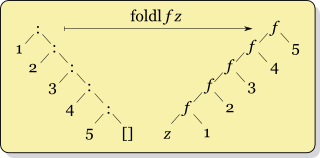
\includegraphics[width=0.5\textwidth]{fold_left}
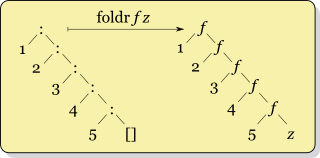
\includegraphics[width=0.5\textwidth]{fold_right}
\caption{Illustrations of fold left and fold right.~\cite{foldl}\cite{foldr}}
\label{fig:folds}
\end{figure}

We will now look into how we could implement this in Coq.

\subsection{Fold right} 
We implement \texttt{fold\_right} by matching on the input list. If the list is
empty, then we return the \texttt{nil\_case}. If the list is a head and a tail,
we apply the \texttt{cons\_case} to the head and call \texttt{fold\_right}
recursively on the tail.

\subsection{Fold left}
We implement \texttt{fold\_left} by matching input list. If the list is empty,
we return the \texttt{nil\_case}. If the list is a head and a tail, we call
\texttt{fold\_left} recursively, where the \texttt{nil\_case} is replaced by
an application of the \texttt{cons\_case} on the head and the former
\texttt{nil\_case}, and the list on which we now do the fold is the tail of the
list.

\section{A few functions}
In this section we will specify, define and implement a few different functions
using \texttt{fold\_right} and \texttt{fold\_left}. This will act as a stepping
stone, while we are learning to better understand \texttt{fold\_right} and
\texttt{fold\_left}.

One should note that all of the following functions could be implemented without
using fold. But when we have the fold mechanism it turns out to be very easy to
implement these functions.

\subsection{List Identity}
We start with the simple example of the \texttt{list\_identity} function. The
\linebreak\texttt{list\_identity} function takes a type and a list of that
type, and returns the list it is given.

We define the \texttt{list\_identity} with \texttt{fold\_right}. The idea is
that we let the \texttt{cons\_case} function be the \texttt{cons} function, and
the \texttt{nil\_case} be \texttt{nil}. In this way any input list would simply
be taken apart and be put back together by the fold.

We prove that it fits the specification with a simple structural induction
proof.

\subsection{List append}
In order to define a \texttt{reverse\_list} function, we will first need an
implementation of \texttt{list\_append}. We will also need
\texttt{list\_append} when we look when we look at the \texttt{map\_append}
function. It happens that we can implement \texttt{list\_append} with fold as
well. The \texttt{list\_append} function takes a type and two lists of that
type, and returns a list where one has been appended on the other.

We implement this almost like the \texttt{list\_identity} function, but this
time we let the \texttt{nil\_case} be the list that we want to append to the
other. This means that the first list is taken apart and constructed with the
\texttt{cons} function, when we reach \texttt{nil}, we replace it by the
\texttt{nil\_case} which is the second list. In turn this gives us exactly what
we want.

Later on in our proofs about \texttt{reverse\_list}, we will need the property
that \texttt{list\_append} is associative, in order to complete the proof. We
prove this property using structural induction on the first list.

\subsection{Reverse list}
With a specification and an implementation of \texttt{list\_append}, we are now
in position to define \texttt{reverse\_list} using fold. The
\texttt{reverse\_list} function takes a type and a list of that type and
returns the reversed list.

This function is actually almost the same as the \texttt{list\_identity}
function. The only difference is that we use \texttt{fold\_left} instead of
\texttt{fold\_right}. This means that we take apart the list and then we
construct it backwards. This in turn gives us the reversed list.

The reason why we needed \texttt{list\_append} is because the specification of
\linebreak \texttt{reverse\_list} relies on \texttt{list\_append}. In fact we
don't need an actual implementation of \texttt{list\_append} at least not in
the proofs about \texttt{reverse\_list}. What we \emph{do} need is the
specification of \texttt{list\_append}. When we have the specification, we can
just make an assumption that we have an implementation, and the use this
assumption to do the proof.

When we prove that this fold implementation of \texttt{reverse\_list} fits the
specification of \texttt{reverse\_list}, we need a master lemma in the
\texttt{cons\_case}. The master lemma is the following property about
\texttt{fold\_left}: having a non-empty list as \texttt{nil\_case} is the
equivalent to letting the \texttt{nil\_case} be \texttt{nil} and then append
the list to the result of the fold. This is proven by structural induction and
with the help of the property that \texttt{list\_append} is associative.

We will see this pattern of using a master lemma in the \texttt{cons\_case} a
few more times in this project.

\subsection{Map}
In order to further explore how folds work, we decided to go a bit beyond the
project and look into \texttt{map} and a variation of it called
\texttt{map\_append}. We start by looking at the ordinary \texttt{map}
function.

\texttt{map} takes two types, a function from the first to the second type and
a list of the first type.  It then returns a list where the function has been
applied to each element of the former list.

We implemented this using \texttt{fold\_right}. We let the \texttt{cons\_case}
of the fold apply the function to the current element, and we use \texttt{cons}
to construct the new list.

\subsection{Map append}
\texttt{map\_append} is a variation of \texttt{map} but where the function it
is given always returns a list. When we use an ordinary \texttt{map}, and the
function that we give it returns a list, then the result of the \texttt{map}
will be a list of lists.  Sometimes we would rather have that we just got a
flattened list back. This is exactly what \texttt{map\_append} achieves.

The implementation looks a lot like the \texttt{map} implementation, but the
key difference is that we in the \texttt{cons\_case} have replaced the list
constructor with our implementation of \texttt{list\_append}. This means that
instead of constructing a list by using \texttt{cons} on lists, we construct a
list by appending lists together. In turn this yields a flattened list instead
of a list of lists.

\section{Back and forth}
In this section we will look at a connection between \texttt{fold\_right} and
\texttt{fold\_left}. We will in turn be able to define each in term of the
other. We will accomplish this with an accumulator.

\subsection{Fold left from fold right}
We implement this by letting the fold have a \texttt{nil\_case} function which
simply returns what it is given. Lets call this function $n$.

\begin{center}
  $n(a) = a$
\end{center}

And the \texttt{cons\_case} function which we will denote with a $c$, looks
like this:

\begin{center}
  $c(x, h, a) = h (cons\_case(x, a))$
\end{center}

Please note that these are the functions we pass to \texttt{fold\_right} as
\texttt{nil\_case} and \texttt{cons\_case}, and the $cons\_case$ mentioned here
is the one we would normally pass to \texttt{fold\_left}. We know from the
specification of folds that they return the same type as their
\texttt{nil\_case}, which means that when we give the above two to
\texttt{fold\_right}, the result will be a function taking one argument just
like the \texttt{nil\_case} function. This turns out to be a perfect fit for
the function $h$.

In order to better explain this, consider the list $cons(1,cons(2, nil))$. 
\begin{align*}
        &fold\_left(nil\_case, cons\_case, cons(1,cons(2, nil))) 
  \\ &= fold\_right(n, c, cons(1,cons(2, nil)))(nil\_case)
  \\ &= (a \rightarrow c(1, fold\_right(n, c, cons(2,nil), a)))(nil\_case)
  \\ &= c(1, fold\_right(n, c, cons(2,nil), nil\_case))
  \\ &= fold\_right(n, c, cons(2,nil))(cons\_case(1,nil\_case))
  \\ &= fold\_right(n, c, nil)(cons\_case(2,cons\_case(1,nil\_case)))
  \\ &= n(cons\_case(2,cons\_case(1,nil\_case)))
  \\ &= cons\_case(2,cons\_case(1,nil\_case))
\end{align*}

In the final line we see that we get exactly what we would expect an ordinary
\texttt{fold\_left} would do.

Proving that this implementation of \texttt{fold\_left} fits the specification,
and thereby always \emph{acts} as a \texttt{fold\_left} is done by a simple
structural induction proof on the input list.

\subsection{Fold right from fold left}
The implementation of \texttt{fold\_right} is very similar to that of the
\texttt{fold\_left} implementation which we just looked at. $n$ and $c$ will
remain the same, and if we do the same example as the one above we get:
\begin{align*}
        &fold\_right(nil\_case, cons\_case, cons(1,cons(2, nil))) 
  \\ &= fold\_left(n, c, cons(1,cons(2, nil)))(nil\_case)
  \\ &= fold\_left((a \rightarrow c(1, n, a)), c, cons(2,nil))(nil\_case)
  \\ &= fold\_left((a \rightarrow n (cons\_case(1, a))), c, cons(2,nil))(nil\_case)
  \\ &= fold\_left((a \rightarrow cons\_case(1, a)), c, cons(2,nil))(nil\_case)
  \\ &= fold\_left((a \rightarrow (a \rightarrow 
  cons\_case(1,a))(cons\_case(2,a))), c, nil)(nil\_case)
  \\ &= (a \rightarrow (a \rightarrow
  cons\_case(1,a))(cons\_case(2,a)))(nil\_case)
  \\ &= (a \rightarrow cons\_case(1,a))(cons\_case(2, nil\_case))
  \\ &= cons\_case(1,cons\_case(2, nil\_case))
\end{align*}

Again we see that the result is what we would expect from a
\texttt{fold\_right}.

In order to prover that this is the case for all lists and not just the one in
the example, we do a proof by structural induction on the list. Where the
\texttt{cons\_case} uses a master lemma.

\section{When cons case is an associative and commutative function}
When we wrote the code for the project, we noticed that some of the unit tests
for \texttt{fold\_right} and \texttt{fold\_left} were identical, and still
passed for both of the functions, while others only passed for one of them.

This happens when the \texttt{cons\_case} is an associative and commutative
function. In order for the \texttt{cons\_case} function to be associative and
commutative, it must take two arguments of the same type. This means that if we
can prove that the \texttt{cons\_case} function is associative and commutative,
then it should make no difference whether we choose to use \texttt{fold\_right}
or \texttt{fold\_left} --- The result should be the same.

When we did the project we started by showing that the property held for
\texttt{plus} as the \texttt{cons\_case} function. We did this as stepping
stone before writing a more generalised version of the property. One should
note that we choose to use \texttt{ring} as the tactic that applies the
associativity, commutativity and neutral element rules. We could have written
it out using the actual lemmas as well. When writing the generalised version,
one sees that the actual proofs are more or less the same thing.

\subsection{Structure of the proof}
The proof consists of a proof by structural induction on the input list.

In the \texttt{cons\_case} we will need a master lemma, which shows that after
applying the \texttt{cons\_case} for each of the folds once,
\texttt{fold\_right} can then be replaced by \texttt{fold\_left}. The master
lemma is also proven by structural induction. It is reasonable to this nested
induction because we will need three values in order to apply the associativity
rules.

The \texttt{cons\_case} of the master lemma is where we actually use the
assumption that the \texttt{cons\_case} function is associative and
commutative, and that is really the core of the proof.

\section{Primitive iteration and primitive recursion over polymorphic lists}
In the course for which this is a term project, we visited primitive recursion
and primitive iteration. In this section we will compare the two with
\texttt{fold\_left} and \texttt{fold\_right}.

The versions of primitive iteration and recursion that we looked at during the
course, worked on natural numbers. In order to compare with \texttt{fold\_left}
and right, we will need to specify and implement new versions of primitive
iteration and primitive recursion. First we will specify
\texttt{p\_i\_over\_polymorphic\_lists} (primitive iteration over polymorphic
lists), and compare this to \texttt{fold\_left} and \texttt{fold\_right}.
Afterwards we will specify \texttt{p\_r\_over\_polymorphic\_lists} (primitive
recursion over polymorphic lists) and do the same thing for that function.

\subsection{Primitive iteration over lists}
When we implement \texttt{p\_i\_over\_polymorphic\_lists}, we must define two
things.
\begin{enumerate}
  \item What to do when the list is empty.
  \item What to do when the list consists of a head and a tail
\end{enumerate}

In the first case, we return what we want to happen when we reach \texttt{nil}.
In the second case, we return the result of applying a \texttt{cons\_case}
function with the head of the list as the first argument and in the second
argument we call \texttt{p\_i\_over\_polymorphic\_lists}.

\subsubsection{Fold right from primitive iteration}
If we at this point stop and look at the specification of \texttt{fold\_right},
we will see that the specifications are in fact the same thing. If we have an
implementation of \texttt{p\_i\_over\_polymorphic\_lists}, we can easily get an
implementation of \texttt{fold\_right} because
\texttt{p\_i\_over\_polymorphic\_lists} also satisfies the specification of
\texttt{fold\_right}.

In fact this means that \texttt{p\_i\_over\_polymorphic\_lists} is the same thing as \texttt{fold\_right}.

\subsubsection{Fold left from primitive iteration} 
We know that \texttt{p\_i\_over\_polymorphic\_lists} satisfies the
specification of \linebreak\texttt{fold\_right} and earlier in the project we
found a way of using a \texttt{fold\_right} to get a \texttt{fold\_left}. If we
combine this knowledge, we will have an implementation of \texttt{fold\_left}
from \texttt{p\_i\_over\_polymorphic\_lists}.

\subsection{Primitive recursion over lists}
\texttt{p\_r\_over\_polymorphic\_lists} is almost like
\texttt{p\_i\_over\_polymorphic\_lists}, only with a slight change to the
\texttt{cons\_case} function. The \texttt{cons\_case} function now takes one
more argument, which is a snapshot of the current list.

We can implement \texttt{fold\_right} and \texttt{fold\_left} in the exact same
way as with \texttt{p\_i\_over\_polymorphic\_lists}, if we just ignore that the
snapshot exists.

\subsubsection{Usage of the snapshot}
This project was focused on folds, and we can easily implement folds without
using the snapshots. But in order to show some example usage of the snapshot in
\texttt{p\_r\_over\_polymorphic\_lists}, we implemented a function which maps a
list to the list of it's suffixes.

The last two unit tests for \texttt{p\_r\_over\_polymorphic\_lists} show two
functions which make use of the snapshots. The first one returns a list of all
the snapshots, the second returns a flattened list of snapshots. 

We took a step further and defined three versions of the
\texttt{list\_of\_suffixes} function (the first one of the two mentioned
above), where one of these use the snapshot like the one in the unit test. The
other two are alternative implementations. We then prove these to be
equivalent.

This is done by structural induction on the input list. When proving the
equivalency with the one that uses \texttt{p\_i\_over\_polymorphic\_lists}, we
need a master lemma. Apart from that the proof is straight forward.

\section{Conclusion}
In this report we looked at \texttt{fold\_right} and \texttt{fold\_left}. We
saw that they share the same expressive power, by showing that one could be
defined in terms of the other. Afterwards we found out that when the
\texttt{cons\_case} function that we pass to a fold function is associative and
commutative, then we get the same result no matter if we use
\texttt{fold\_left} or \texttt{fold\_right}. 

During this we saw a recurring proof pattern where we in the induction case of a
structural induction proof, needed a master lemma in order to complete the
proof.

In the end we saw that \texttt{p\_i\_over\_polymorphic\_lists} is the exact
same thing as \texttt{fold\_right}. Using the connection between
\texttt{fold\_right} and \texttt{fold\_left}, we were able to define \texttt{fold\_left} in terms
of \texttt{p\_i\_over\_polymorphic\_lists}. We also saw how the snapshot in \texttt{p\_r\_over\_polymorphic\_lists} was
irrelevant in relation to folding.

\printbibliography[heading=bibnumbered]{}

\end{document}
